\documentclass[tikz,border=5pt]{standalone}
\usepackage{amsmath}
\usepackage{xcolor}
\usetikzlibrary{arrows.meta,calc}

\definecolor{Ink}{HTML}{1F2937}
\definecolor{Slate}{HTML}{334155}
\definecolor{InputFill}{HTML}{EAF3FB}
\definecolor{InputDraw}{HTML}{829DB4}
\definecolor{BaselineFill}{HTML}{EEF2F6}
\definecolor{BaselineDraw}{HTML}{8795A5}
\definecolor{ResidualFill}{HTML}{FFF3DA}
\definecolor{ResidualDraw}{HTML}{B49B63}
\definecolor{TealFill}{HTML}{E7F3EF}
\definecolor{TealDraw}{HTML}{6B9D92}
\definecolor{TealArrow}{HTML}{227C70}
\definecolor{EvaluationFill}{HTML}{F1EFF6}
\definecolor{EvaluationDraw}{HTML}{9892A5}
\definecolor{NoteGray}{HTML}{4B5563}

\newcommand{\nodeheading}[1]{%
  {\sffamily\fontsize{9.5}{11.3}\selectfont\bfseries #1}%
}

\pagecolor{white}

\begin{document}
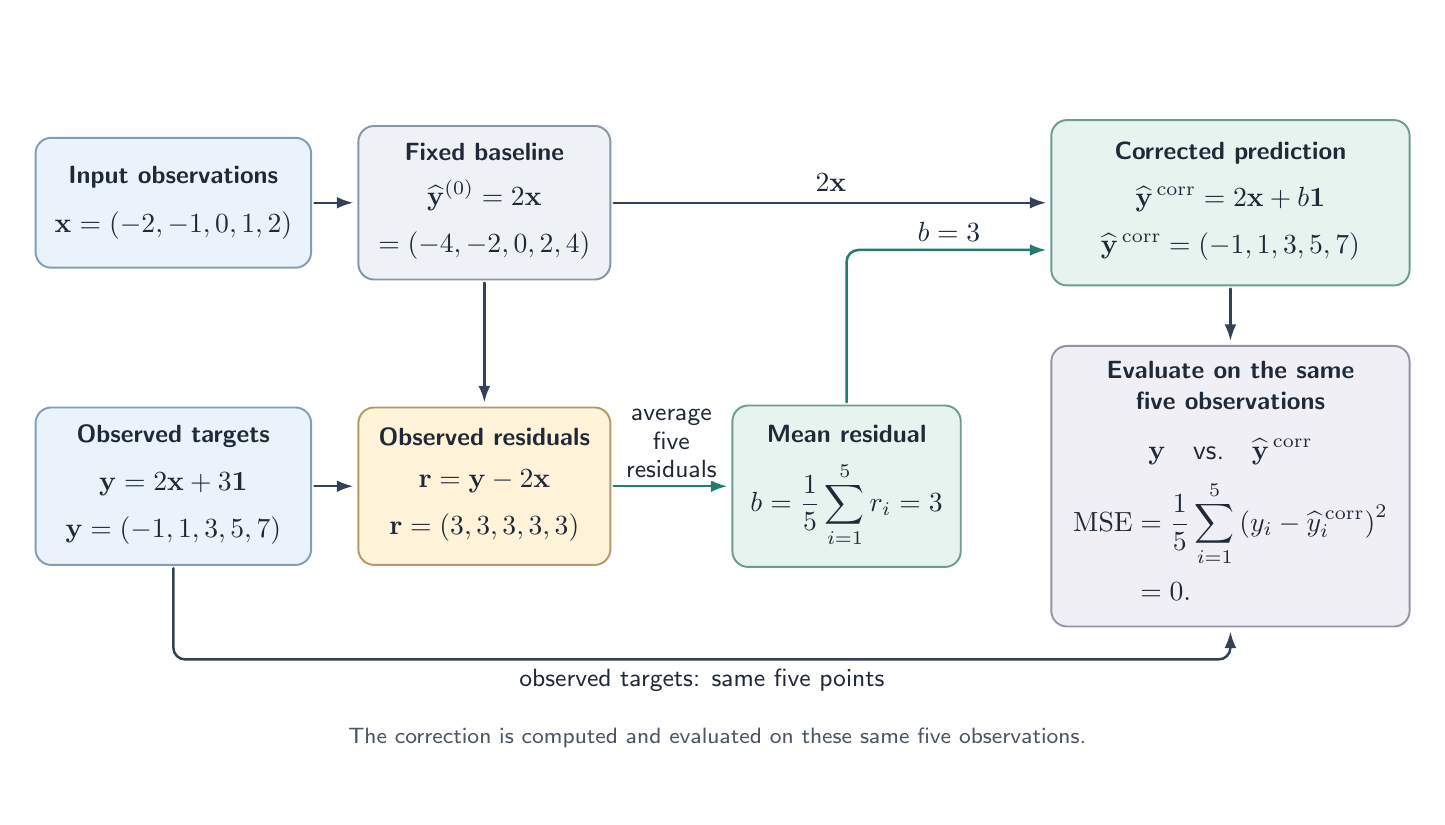
\begin{tikzpicture}[
  x=1cm,
  y=1cm,
  box/.style={
    rectangle,
    rounded corners=2mm,
    line width=0.7pt,
    inner xsep=2mm,
    inner ysep=2mm,
    outer sep=0pt,
    align=center,
    text=Ink,
    font=\sffamily\fontsize{10}{12}\selectfont
  },
  supplied/.style={
    box,
    fill=InputFill,
    draw=InputDraw,
    minimum width=3.50cm,
    text width=3.10cm
  },
  baselinebox/.style={
    box,
    fill=BaselineFill,
    draw=BaselineDraw,
    minimum width=3.20cm,
    text width=2.80cm
  },
  residualbox/.style={
    box,
    fill=ResidualFill,
    draw=ResidualDraw,
    minimum width=3.20cm,
    text width=2.80cm
  },
  meanbox/.style={
    box,
    fill=TealFill,
    draw=TealDraw,
    minimum width=2.90cm,
    text width=2.50cm
  },
  predictionbox/.style={
    box,
    fill=TealFill,
    draw=TealDraw,
    minimum width=4.55cm,
    text width=4.15cm
  },
  evaluationbox/.style={
    box,
    fill=EvaluationFill,
    draw=EvaluationDraw,
    minimum width=4.55cm,
    text width=4.15cm
  },
  dependency/.style={
    draw=Slate,
    line width=0.9pt,
    solid,
    line cap=round,
    line join=round,
    -{Latex[length=2.1mm,width=1.5mm]},
    shorten <=1.2pt,
    shorten >=1.8pt
  },
  correction/.style={
    dependency,
    draw=TealArrow
  },
  arrowlabel/.style={
    text=Ink,
    fill=white,
    inner sep=1.2pt,
    outer sep=0pt,
    align=center,
    font=\sffamily\fontsize{9}{10.2}\selectfont
  },
  mathlabel/.style={
    arrowlabel,
    font=\fontsize{10}{12}\selectfont
  }
]

% Including the standalone border, the page is 18 cm by 10.125 cm (16:9).
% The schematic itself occupies approximately 18 cm by 8 cm.
\pgfmathsetlengthmacro{\canvaswidth}{18cm-10pt}
\pgfmathsetlengthmacro{\canvasheight}{10.125cm-10pt}
\path[use as bounding box,fill=white]
  (0,0) rectangle (\canvaswidth,\canvasheight);

% Upper row.
\node[supplied,minimum height=1.65cm] (inputs) at (1.85,7.55) {
  \nodeheading{Input observations}\\[6pt]
  \(\displaystyle \mathbf{x}=(-2,-1,0,1,2)\)
};

\node[baselinebox,minimum height=1.95cm] (baseline) at (5.80,7.55) {
  \nodeheading{Fixed baseline}\\[6pt]
  \(\displaystyle
    \begin{gathered}
      \widehat{\mathbf{y}}^{(0)}=2\mathbf{x}\\[2pt]
      =(-4,-2,0,2,4)
    \end{gathered}
  \)
};

\node[predictionbox,minimum height=2.10cm] (corrected) at (15.275,7.55) {
  \nodeheading{Corrected prediction}\\[6pt]
  \(\displaystyle
    \begin{gathered}
      \widehat{\mathbf{y}}^{\,\mathrm{corr}}
        =2\mathbf{x}+b\mathbf{1}\\[2pt]
      \widehat{\mathbf{y}}^{\,\mathrm{corr}}
        =(-1,1,3,5,7)
    \end{gathered}
  \)
};

% Lower row.
\node[supplied,minimum height=2.00cm] (targets) at (1.85,3.95) {
  \nodeheading{Observed targets}\\[6pt]
  \(\displaystyle
    \begin{gathered}
      \mathbf{y}=2\mathbf{x}+3\mathbf{1}\\[2pt]
      \mathbf{y}=(-1,1,3,5,7)
    \end{gathered}
  \)
};

\node[residualbox,minimum height=2.00cm] (residuals) at (5.80,3.95) {
  \nodeheading{Observed residuals}\\[6pt]
  \(\displaystyle
    \begin{gathered}
      \mathbf{r}=\mathbf{y}-2\mathbf{x}\\[2pt]
      \mathbf{r}=(3,3,3,3,3)
    \end{gathered}
  \)
};

\node[meanbox,minimum height=2.05cm] (mean) at (10.40,3.95) {
  \nodeheading{Mean residual}\\[6pt]
  \(\displaystyle b=\frac{1}{5}\sum_{i=1}^{5}r_i=3\)
};

\node[evaluationbox,minimum height=3.50cm] (evaluation) at (15.275,3.95) {
  \nodeheading{Evaluate on the same\\[-1pt]five observations}\\[6pt]
  \(\displaystyle
    \mathbf{y}\quad\text{vs.}\quad
    \widehat{\mathbf{y}}^{\,\mathrm{corr}}
  \)\\[5pt]
  \(\displaystyle
    \begin{aligned}
      \mathrm{MSE}
        &=\frac{1}{5}\sum_{i=1}^{5}
          \left(y_i-\widehat y_i^{\,\mathrm{corr}}\right)^2\\
        &=0.
    \end{aligned}
  \)
};

% 1. Inputs to fixed baseline.
\draw[dependency]
  (inputs.east) -- (baseline.west);

% 2. Fixed baseline to observed residuals.
\draw[dependency]
  (baseline.south) -- (residuals.north);

% 3. Observed targets to observed residuals.
\draw[dependency]
  (targets.east) -- (residuals.west);

% 4. Residuals to their scalar mean.
\draw[correction]
  (residuals.east) --
  node[midway,above=2pt,arrowlabel,text width=1.30cm]
    {average\\five\\residuals}
  (mean.west);

% 5. Baseline prediction through the open upper third column.
\draw[dependency]
  (baseline.east) --
  node[midway,above=3pt,mathlabel] {\(2\mathbf{x}\)}
  (corrected.west);

% 6. Mean correction enters a separate, lower prediction port.
\coordinate (correctionport) at ($(corrected.west)+(0,-0.60)$);
\draw[correction,rounded corners=1.5mm]
  (mean.north) --
  (10.40,6.95) --
  node[midway,above=2pt,mathlabel] {\(b=3\)}
  (correctionport);

% 7. Corrected prediction to evaluation.
\draw[dependency]
  (corrected.south) -- (evaluation.north);

% 8. Target data travel through a dedicated channel below the lower row.
\draw[dependency,rounded corners=1.5mm]
  (targets.south) --
  (1.85,1.75) --
  node[midway,below=2.5pt,arrowlabel]
    {observed targets: same five points}
  (15.275,1.75) --
  (evaluation.south);

\node[
  text=NoteGray,
  align=center,
  inner sep=0pt,
  outer sep=0pt,
  font=\sffamily\fontsize{8.5}{10.2}\selectfont
] at (8.824,0.75) {
  The correction is computed and evaluated on these same five observations.
};

\end{tikzpicture}
\end{document}